($\Leftarrow$) \underline{Claim} Every triple $\left( x,\,y,\,z \right)$ with
$x=m^2-n^2$, $y=2mn$, $z=m^2+n^2$ where $m,\,n\in\mathbb{Z}^+$, $m>n$ ($m$: even, $n$: odd)
or ($m$: odd, $n$: even) and $\left( m,\,n \right)=1$ is a primitive pythagorean triple.
Clearly $\left( x,\,y,\,z \right)$ is a pythagorean triple.

We want to show that $\left( x,\,y,\,z \right)=1$. Suppose $\left( x,\,y,\,z \right)=d>1$,
then $\exists$ prime $p$ with $p \divides \left( x,\,y,\,z \right)$.
Note that $p\neq 2$ since $x$ is odd.

Since $p \divides x$ and $p \divides z$,
\begin{align*}
    p \divides \left(x+z\right) & \quad \mbox{ and so } \quad p\divides 2m^2,\\
    p \divides \left(x-z\right) & \quad \mbox{ and so } \quad p\divides 2n^2.
\end{align*}
Thus $p \divides m^2$ and $p \divides n^2$, and so $p \divides m$ and $p \divides n$.
$\rightarrow\leftarrow$

\begin{remark}
    \begin{enumerate}
        \item $a^2+b^2=c^2$, $c \neq 0$, $a,\,b,\,c\in\mathbb{Z}$
        $\Rightarrow$ $\left(\frac{a}{c}\right)^2+\left(\frac{b}{c}\right)^2=1$.

        Conversely, by choosing the least common denominator, we can write $x=\frac{a}{c}$, $y=\frac{b}{c}$,
        then $1=x_0^2+y_0^2=\left(\frac{a}{c}\right)^2+\left(\frac{b}{c}\right)^2$ and so $a^2+b^2=c^2$.
        \item Consider
        \begin{center}
            \begin{tikzpicture}
                \tikzset{>=stealth}
                \draw[->] (-4,0) -- ++(8,0) coordinate (X) node[below] {$x$};
                \draw[->] (0,-4) -- ++(0,8) node[left] {$y$};

                \draw (-4,-0.5) -- ++(7,3.5) node[right] {$y=t\left(x+1\right)$};
                \draw (-3,0) node[above left] {$-1$};
                \draw (3,0) node[below right] {$1$};
                \draw (0,3) node[above right] {$1$};
                \draw (0,-3) node[below right] {$-1$};
                \draw (0,0) node[below right] {$\mathrm{O}$};
                \draw (2,-2) node[below right] {$x^2+y^2=1$};
                \draw (1.8,2.4) node[above] {$\left( x,\,y \right)$};

                \draw (0,0) circle (3cm);
                \draw[fill=black] (1.8,2.4) circle (0.05cm);
                \draw[fill=black] (-3,0) circle (0.05cm);
            \end{tikzpicture}
        \end{center}
        Note that
        \[
            x^2+\left(t\left(x+1\right)\right)^2=1
        \]
        then
        \begin{align*}
            & x^2-1+t^2\left(x+1\right)^2=0 \\
            &\Rightarrow \left(x+1\right)\left(\left(x-1\right)+t^2\left(x+1\right)\right)=0 \\
            &\Rightarrow x-1+t^2x+t^2=0 \\
            &\Rightarrow x=\frac{1-t^2}{1+t^2} \quad \mbox{and so} \quad y=\frac{2t}{1+t^2}.
        \end{align*}
        If we take $t=\frac{n}{m}$, then 
        \[
            \left( \frac{1-t^2}{1+t^2},\,\frac{2t}{1+t^2} \right) = \left( \frac{m^2-n^2}{m^2+n^2},\,\frac{2mn}{m^2+n^2} \right).
        \]
    \end{enumerate}
\end{remark}

\begin{theorem}
    $x^4+y^4=z^4$ has no nontrivial solutions.
\end{theorem}

\begin{proof}
    (Proof shown in next class.)
\end{proof}

\begin{definition}[Congrugent Numbers]
    $n \in \mathbb{Z}^+$. $n$ is said to be a \textbf{congrugent number}
    if $\exists a,\,b,\,c \in \mathbb{Q}$ such that $a^2+b^2=c^2$ and $\frac{1}{2}ab=n$.
\end{definition}

e. g. 

\begin{center}
    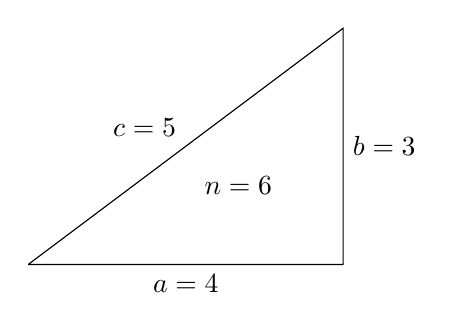
\begin{tikzpicture}
        \tikzset{>=stealth}
        \draw (0,0) -- (4,0) -- (4,3) -- (0,0);
        \draw (2,0) node[below] {$a=4$};
        \draw (4,1.5) node[right] {$b=3$};
        \draw (2,1.5) node[above left] {$c=5$};
        \draw (8/3,1) node {$n=6$};
    \end{tikzpicture}
\end{center}

\begin{center}
    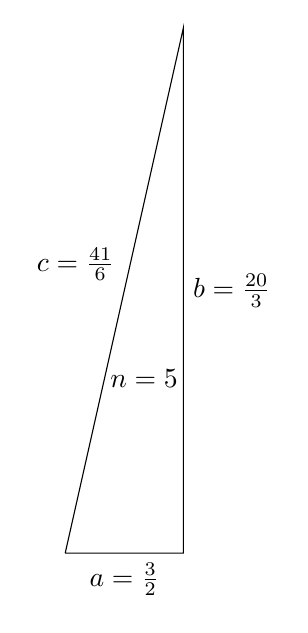
\begin{tikzpicture}
        \tikzset{>=stealth}
        \draw (0,0) -- (3/2,0) -- (3/2,20/3) -- (0,0);
        \draw (3/4,0) node[below] {$a=\frac{3}{2}$};
        \draw (3/2,10/3) node[right] {$b=\frac{20}{3}$};
        \draw (3/4,10/3) node[above left] {$c=\frac{41}{6}$};
        \draw (1,20/9) node {$n=5$};
    \end{tikzpicture}
\end{center}

Fermat showed that 1, 2, 3 are not congrugent numbers.

\paragraph{cf)} Suffice to consider the case when $n$ is square-free
in order to solve the congrugent number problem.

\paragraph{Conjecture} $n\equiv 5,\,6,\,7\pmod{8}\Rightarrow n$
is a congrugent number.

\begin{remark}
    If Birch and Swinnerton-Dyer Conjecture is a theorem,
    then the conjecture of congrugent number also holds.
\end{remark}

\paragraph{Question} Are there 3 consecutive integers whose product
is a perfect square?

Consider $y^2=x\left(x+1\right)\left(x+2\right)$. It is known that
there are no integer solutions other tha trivial ones.
Moreover, it is known that there are no nontrivial rational solutions.

\paragraph{Question} Are there three integers that differ by 5 whose
product is a perfect square? i. e. $y^2=x\left(x+5\right)\left(x+10\right)$.

As in the previous one, $\exists$ trivial solutions $\left( 0,\,0 \right)$,
$\left( -5,\,0 \right)$, $\left( -10,\,0 \right)$. But in this case there are
nontrivial ones. e. g.:
$\left(-9\right)\left(-9+5\right)\left(-9+10\right)=-9\cdot-4\cdot 1=6^2$.
Moreover, there are also rational solutions which are far from obvious:
$\left(\frac{4}{5}\right)\left(\frac{5}{4}+5\right)\left(\frac{5}{4}+10\right)=\left(\frac{75}{8}\right)^2$.
In fact, there are infinitely many rational solutions of this equation.

\begin{definition}
    An \textbf{elliptic curve} is a curve of the form
    \[y^2=x^3+ax+b\]
    where $a,\,b\in\mathbb{Z}$ and $\Delta=-16\left(4a^3+27b^2\right)\neq 0$.
\end{definition}

e. g. $y^2=x^3-x$

\begin{center}
    \begin{tikzpicture}
        \begin{axis} [axis lines=center]
            \addplot [domain=-1:0,smooth,thick,samples=200] { sqrt(x^3-x) };
            \addplot [domain=-1:0,smooth,thick,samples=200] { -sqrt(x^3-x) };
            \addplot [domain=1:3,smooth,thick,samples=200] { sqrt(x^3-x) };
            \addplot [domain=1:3,smooth,thick,samples=200] { -sqrt(x^3-x) };
        \end{axis}
    \end{tikzpicture}
\end{center}

$y^2=x^3-x+1$

\begin{center}
    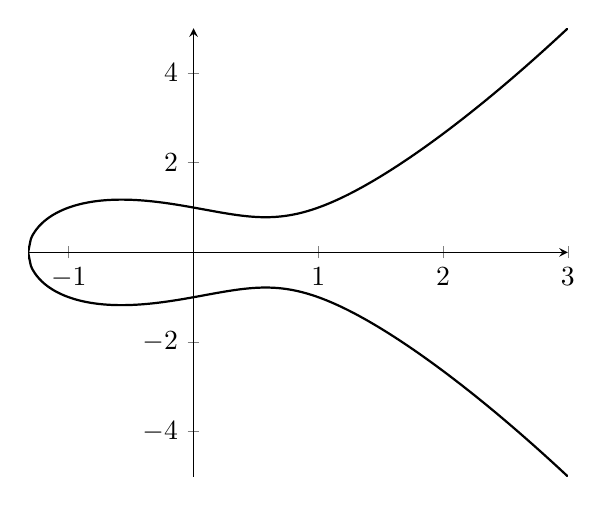
\begin{tikzpicture}
        \begin{axis} [axis lines=center]
            \addplot [domain=-1.3247:3,smooth,thick,samples=200] { sqrt(x^3-x+1) };
            \addplot [domain=-1.3247:3,smooth,thick,samples=200] { -sqrt(x^3-x+1) };
        \end{axis}
    \end{tikzpicture}
\end{center}